
\documentclass{article}

% required packages
\usepackage[usenames,dvipsnames]{color}
\usepackage[nottoc,notlot,notlof]{tocbibind}
\usepackage[toc]{glossaries}
\usepackage{amsmath}
\usepackage{listings} 
\usepackage{graphicx}
\usepackage{wrapfig}
\usepackage{url}

\definecolor{grey}{rgb}{0.9,0.9,0.9}
\lstset{%
basicstyle=\footnotesize,
backgroundcolor=\color{grey},}

\title{Commodore 64}
\author{CSC 350 - Project 1 \\ Daniel Savage - V00701453}
\date{January/February 2014}

\begin{document}
   \maketitle
   
\pagebreak{}

\tableofcontents

\pagebreak{}
   
\section{Introduction}
\paragraph{}
In August of 1982, Commodore International released the Commodore 64, a computer running the 8-bit MOS 6502 architecture. Throughout the 1980's the Commodore 64 was the one of the most prominent home computers of its time, selling over ten million units in its lifetime. The Commodore 64 proved to produce a wide software platform, including productivity tools and rich media applications, such as games. It's wide set of peripherals, including printers, cassette devices, floppy drives, and joysticks made it a comprehensive computing platform for the home user, and software flexibility made it practical for the hobbyist computer enthusiast. Interestingly enough, after it's discontinuation in 1994, the Commodore 64 still enjoys a small, devoted following of enthusiasts, interested in still writing programs for the device.

\begin{figure}[h!]
  \centering
    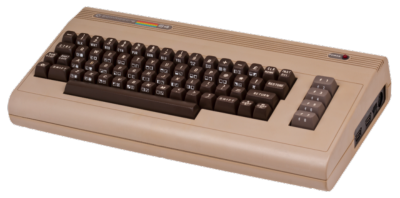
\includegraphics[width=0.8\textwidth]{c64_image}
  \caption{The Commodore 64.}
\end{figure}

\paragraph{}
This document is aimed for computer science students and computer enthusiasts who have a general understanding of computer hardware and some of its general terms. As this document is intended to be short and interesting, the writer of it has asked himself whether or not information organized for this document could keep another computer science student entertained at a cocktail party. If the writer felt it could, then he has included it.

\section{The architecture}

\subsection{Overview}
\paragraph{}
The Commodore 64 consists of a single board, housed in plastic. To many enthusiasts, what defines the Commodore 64 compared to other computers of similar architectures is its unique configuration particular chips. What typically defines the Commodore 64 can typically considered to be the following:
\begin{itemize}
\item The MOS Technology 6510 CPU
\item The MOS Technology 6567 VIC-II
\item The MOS Technology 6581 SID
\item The MOS Technology 6526 CIAx2
\end{itemize}
\paragraph{}
This section will attempt to provide an overview of the system memory, each of these devices, and how they interact with each other in a high-level fashion.

\subsection{Memory}
\paragraph{}
The Commodore 64's CPU has a 16-bit address space, allowing for 64KiB of possible addresses, although various RAM, ROM, and I/O devices are mapped to the same address space. Access to the various spaces on the Commodore 64 happens through bank switching various device lines. This section will give a brief description of each memory device in general, their typical purpose, and also a map of their locations in address space. Throughout the course of this document we will refer to sections of memory in their hexadecimal format. For example, the entire range of the 16-bit address space can be represented as $\mathtt{\$0000 - \$FFFF}$.

\subsubsection{RAM}
\paragraph{}
The Commodore 64 ships with 64KiB of DRAM. Various iterations of the device use different chip layouts from different manufacturers, but are otherwise functionally identical. The refresh rate of the DRAM is controlled by the VIC-II video chip, as it operates the system bus' clock.

\subsubsection{ROM}
\paragraph{}
\begin{wrapfigure}{l}{0.4\textwidth}
\begin{center}
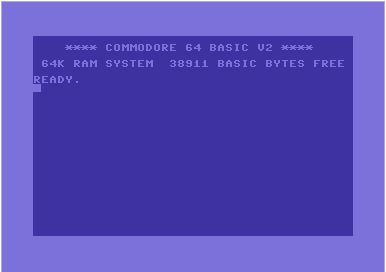
\includegraphics[width=5cm]{c64_basic}
\end{center}
\caption{Commodore BASIC startup screen}
\end{wrapfigure}
There are three pieces of ROM wired to the Commodore 64: the system KERNAL, a CHARACTER ROM table, and a BASIC interpreter; the latter of the two available to the user. The system KERNAL (locations $\mathtt{\$E000 - \$FFFF}$) serves essentially as a core operating system to the user, and provides low-level management of hardware functionality. The CHARACTER ROM (locations $\mathtt{\$D000 - \$DFFF}$) served as default glyph information for the KERNAL and VIC-II video chip to display text. If the programmer desired, they could use the address space RAM for character glyphs instead of ROM, allowing for custom or modified symbols. Lastly, the Commodore 64 also contained a Commodore BASIC interpreter (locations $\mathtt{\$A000 - \$BFFF}$) on the device. Programs written in BASIC only had 38KiB of memory available to them due to the space taken up by the interpreter, as well as tended to be slower than their assembler counterparts, due to the time transferring between RAM and ROM.

\subsubsection{Color RAM}
\paragraph{}
The Commodore 64 can colour characters in its on-screen display by using the system's built-in Color RAM. The Color RAM is 1KB in size, and the first nibble of each byte is used to determine the colour of of each character. Colours are determined with the Commodore 64's built-in fixed colour palette, consisting of 16 possible colours. A programmer wishing to change Color RAM data in Commodore BASIC would often modify the values through the $\mathtt{POKE}$ command, while someone using assembly would need to address the particular section in memory. Color RAM is mapped to locations $\mathtt{\$D800 - \$DBFF}$, when the I/O devices are mapped to memory.

\subsubsection{Memory Map}
\begin{figure}[h!]
  \centering
    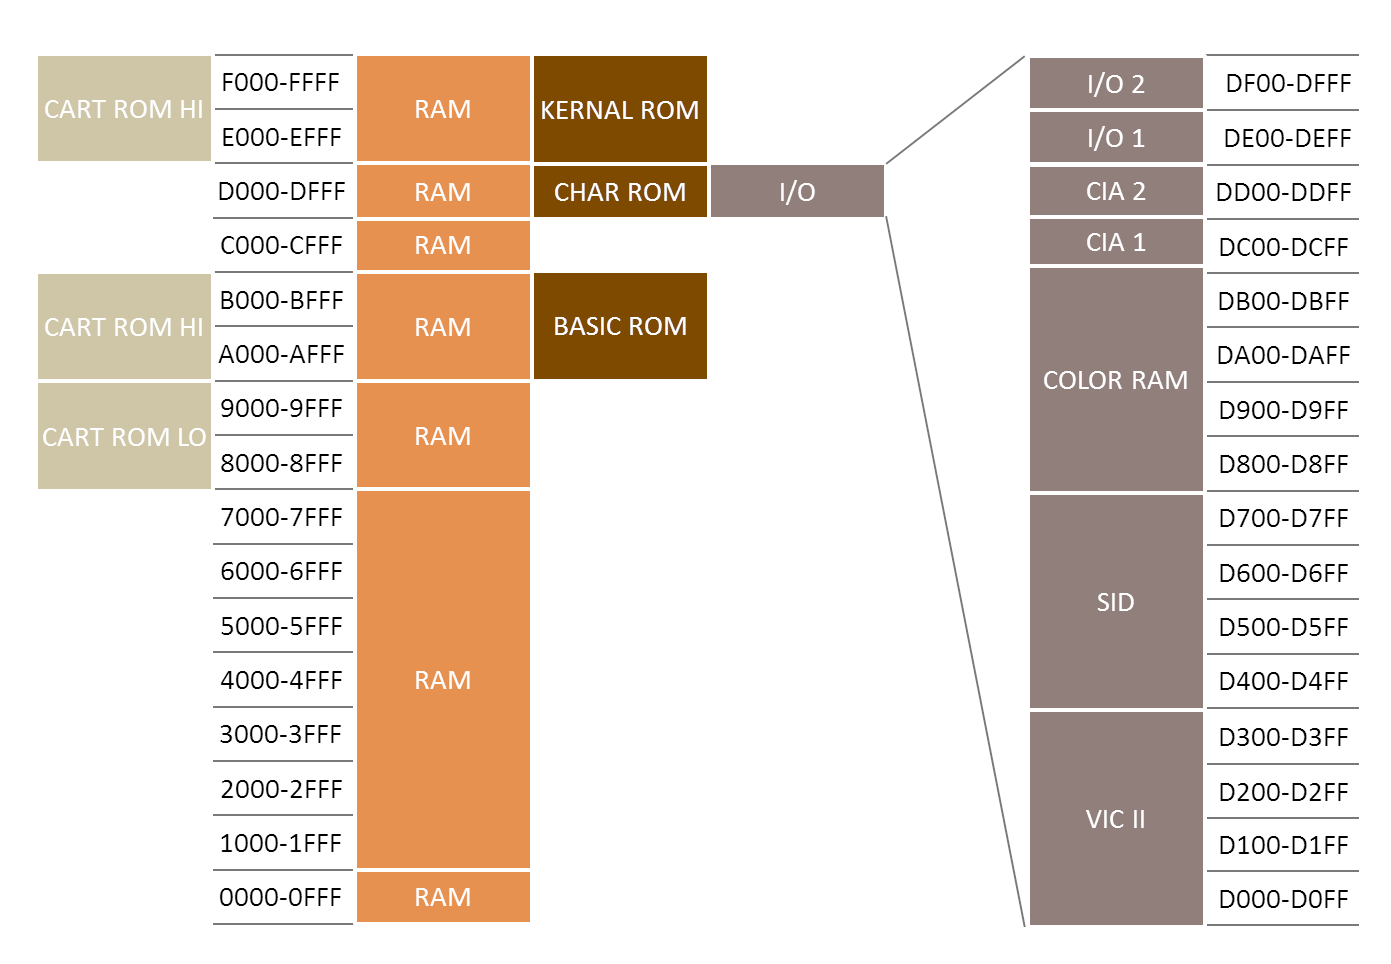
\includegraphics[width=\textwidth]{memmap}
  \caption{The Commodore 64 memory mapping. Each column shows the various address spaces that can be activated and deactivated through bank switching. Source: \cite{memMap}}
\end{figure}

\subsection{MOS 6510 CPU}
\paragraph{}
The Commodore 64's microprocessor is the MOS Technology 6510, a variant of the 6502 model. Leading up to the years of the Commodore 64's production, the MOS 6502 had become substantially popular in consumer computer architecture for its comprehensive features while having a fraction of the price of its competitors. This section will describe the Commodore 64's 6510 in two sections. The first being its general features that is has in common with with the 6502, and the second being its unique characteristics.

\subsubsection{6502 Family Features}

\paragraph{}
The MOS Technology 6502 is a little-endian 8-bit microprocessor with a 16-bit address bus. The 6502 was designed with a two-phase clock design, implementing a very primitive form of pipelining. While an address can be accessed during the first clock phase of the 6502, data can be retrieved during the second from a previous access, allowing two instructions to happen somewhat asynchronously. 

\paragraph{}
The 6502's design can be considered quite minimalistic compared to other designs of its time, such as the Intel 8080. Taking advantage of the fact that memory speeds were much faster CPU clocks at the time of production, the architecture focuses on storing data outside of the processor. Most programming techniques focus on having an accumulator register that is manipulated with various elements from memory. The 6502 has only seven registers: the accumulator (A), two index registers (X, Y), a status register (P), stack pointer (SP), and a double-width, 16-bit program counter (PC). The address space of the stack exists over $\mathtt{\$0100 - \$01FF}$, giving 256 bytes for programming. 

\paragraph{}
The 6502 assembly language is often considered \textit{fun} compared to other varieties of instructions, such as x86. This can often be attributed to the fact that it was inherently designed to be programmed by hand, and less so by an automated compiler. Instructions more or less focus on exchanging or modifying the accumulator with some location in memory, making very straightforward code. A table of common opcodes can be seen here:
    \begin{center}
    \begin{tabular}{|p{2cm}|p{5cm}|p{2cm}|p{5cm}|}
    \hline
    OPCODE & FUNCTION                                       & OPCODE & FUNCTION                                                   \\ \hline
    LDA \#00       & put an immediate value into the accumulator    & ADC \$0110     & add a value from memory into the accumulator with carry    \\ \hline
    LDA \$0110     & load a value from memory into the accumulator  & SBC \$0111     & subtract a value from memory from the accumulator          \\ \hline
    STA \$0111     & store a value from memory into the accumulator & AND \$10       & logical AND function with either memory or immediate value \\ \hline
    LDX \#00       & put an immediate value into the X register     & CMP \$0112     & compare memory and the accumulator                         \\ \hline
    \end{tabular}
    \end{center}

\paragraph{}
An example program is listed below, which doubles a number in the accumulator until it is greater than a specified number in the X register.

\begin{lstlisting}
LDA #01 ; put an unsigned value of 1 into the accumulator
STA $0200 ; store the value in memory
LDX #100 ; put an unsigned limit of 100 into the X register
double: 
LDA $0200 ; load from memory
ADC $0200 ; add the value to itself
STA $0200 ; store the new sum back into memory
CPX $0200 ; compare the value with X
BCC double ; double again until the value is no longer less than X
\end{lstlisting}

\paragraph{}
The 6502 family of microprocessors also has a form of fast zero page addressing modes. Addresses $\mathtt{\$00FF - \$00FF}$ only required a single byte to query memory, allowing for faster access. Zero page addressing could be applied by the assembly programmer by specifying address size as follows.
\begin{lstlisting}
LDA $0F ; load memory $000F using zero page addressing (faster)
LDA $000F ; load memory $000F using normal addressing (slower)
\end{lstlisting}

\subsubsection{6510 Specific Features}
\paragraph{}
\begin{wrapfigure}{l}{0.35\textwidth}
\vspace{-20pt}
\begin{center}
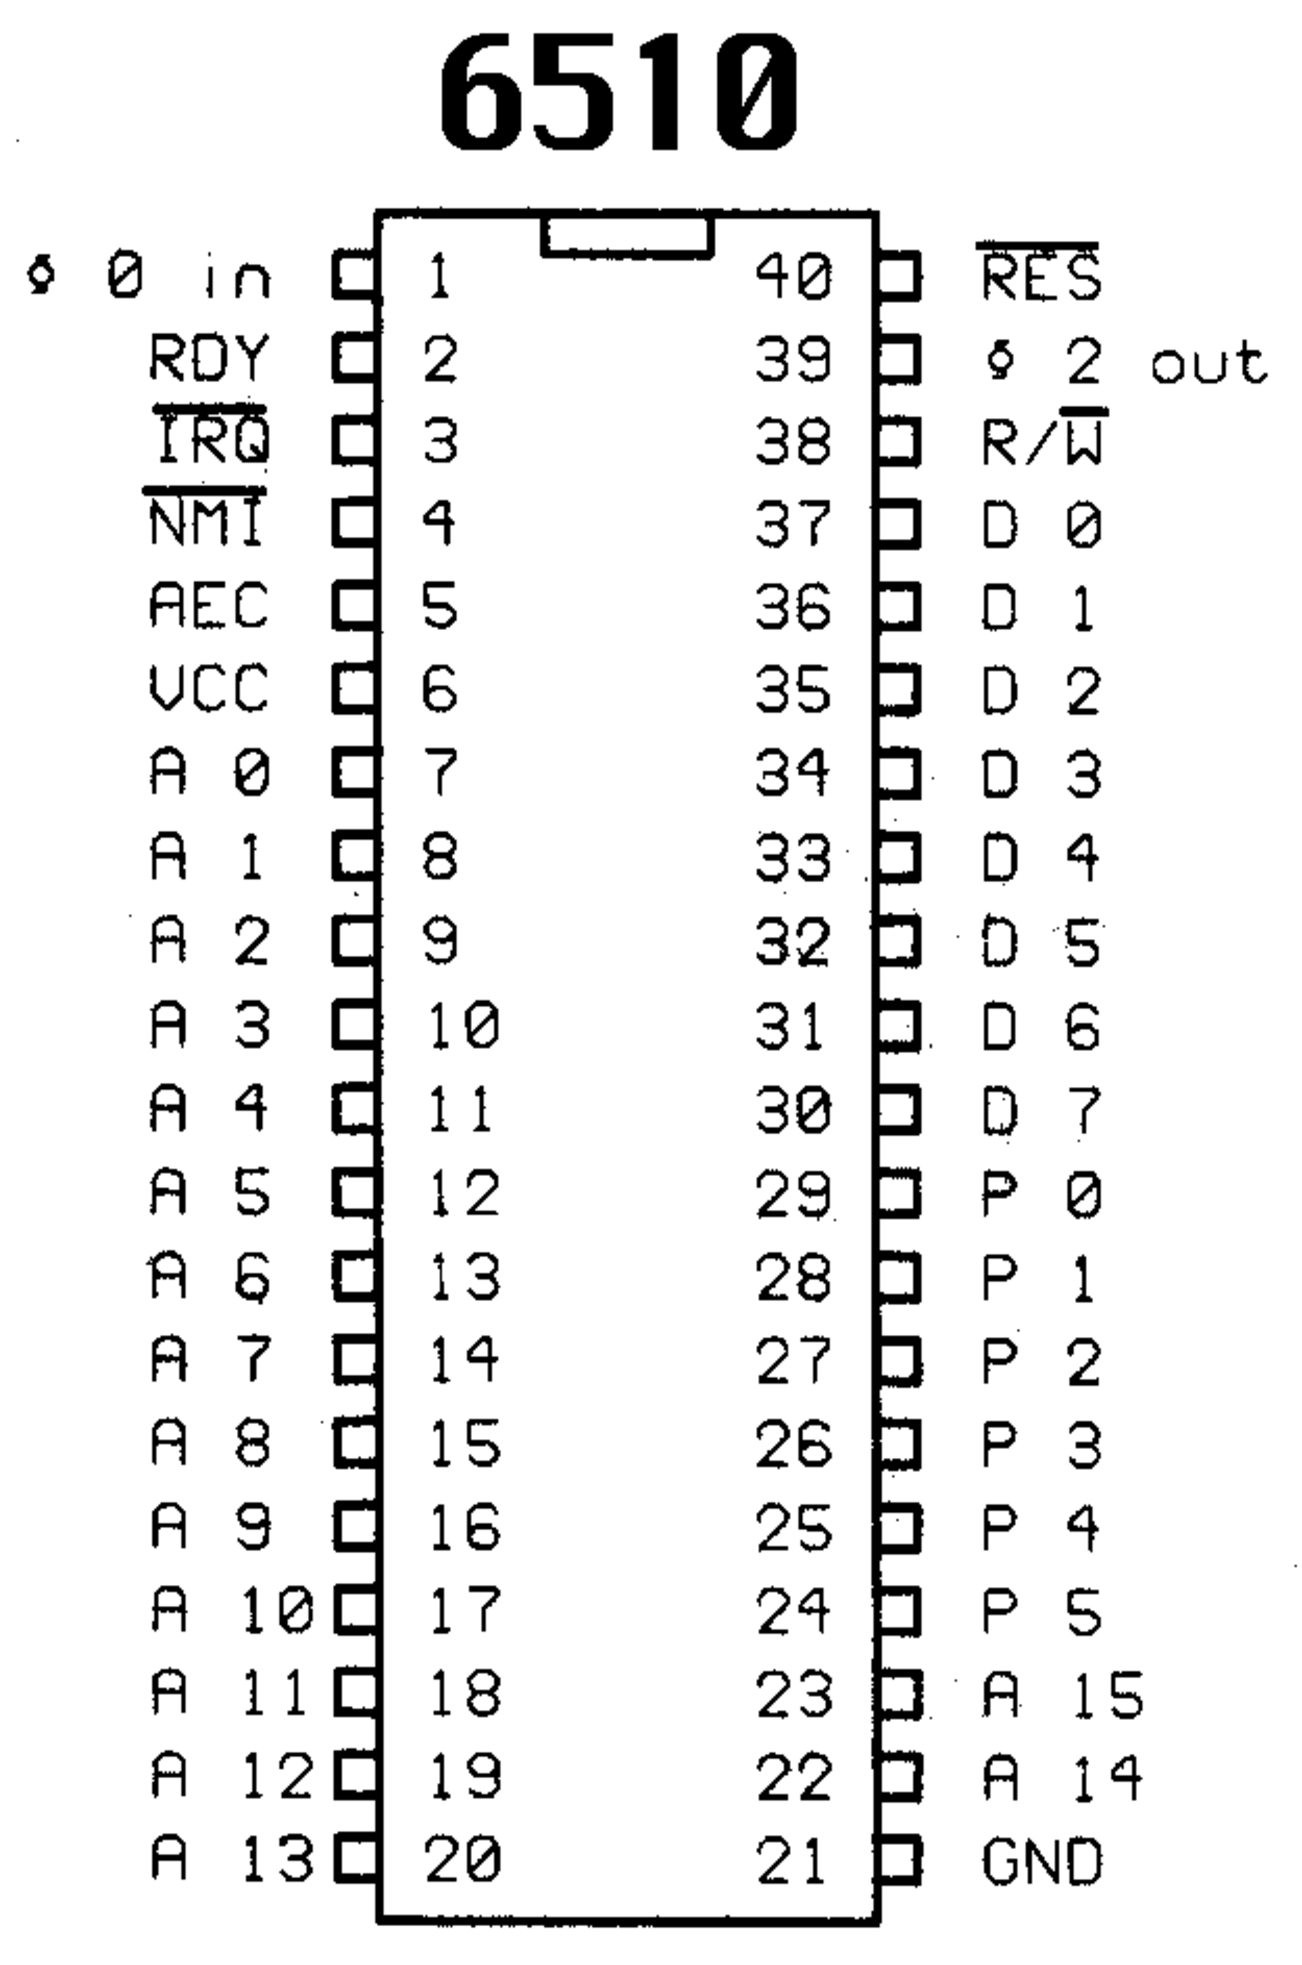
\includegraphics[width=3cm]{6510}
\caption{6510 pin layout. Source: \cite{c64_tech_details}}
\end{center}
\end{wrapfigure}
The MOS Technology 6510 is a variant of the 6502 microprocessor, accompanied with an I/O port of either six or eight bits wide. The Commodore 64 uses the 6-bit version of this port to interact switch between RAM and ROM, as well as access to tertiary memory, such as a datacasette. The 6510 can also make its address lines become tristate, allowing it to share memory with other devices, such as the SID and the VIC-II. Since RAM, ROM, and I/O registers are all mapped to the same address space, the Commodore 64 can distinguish between the three through the $P0$ and $P1$ lines for accessing ROM and external registers on the SID, CIAs and VIC-II, and the $P2$ line for the I/O registers. $P3$, $P4$, and $P5$ are used to operate a datacasette.

\paragraph{}
The 6510 operates around 1MHz, with particular differences whether or not it is within a PAL or NTSC model. There are also a number of variants of the 6510, which were used in later models or other Commodore 64 peripherals. A common example, in particular, being the 8502, which operates at 2 MHz, and the 6510T that uses all 8-bits for its I/O lines inside the Commodore 1551 Disk Drive.

\subsection{MOS 6567 VIC-II}
\paragraph{}
\begin{wrapfigure}{l}{0.35\textwidth}
\vspace{-20pt}
\begin{center}
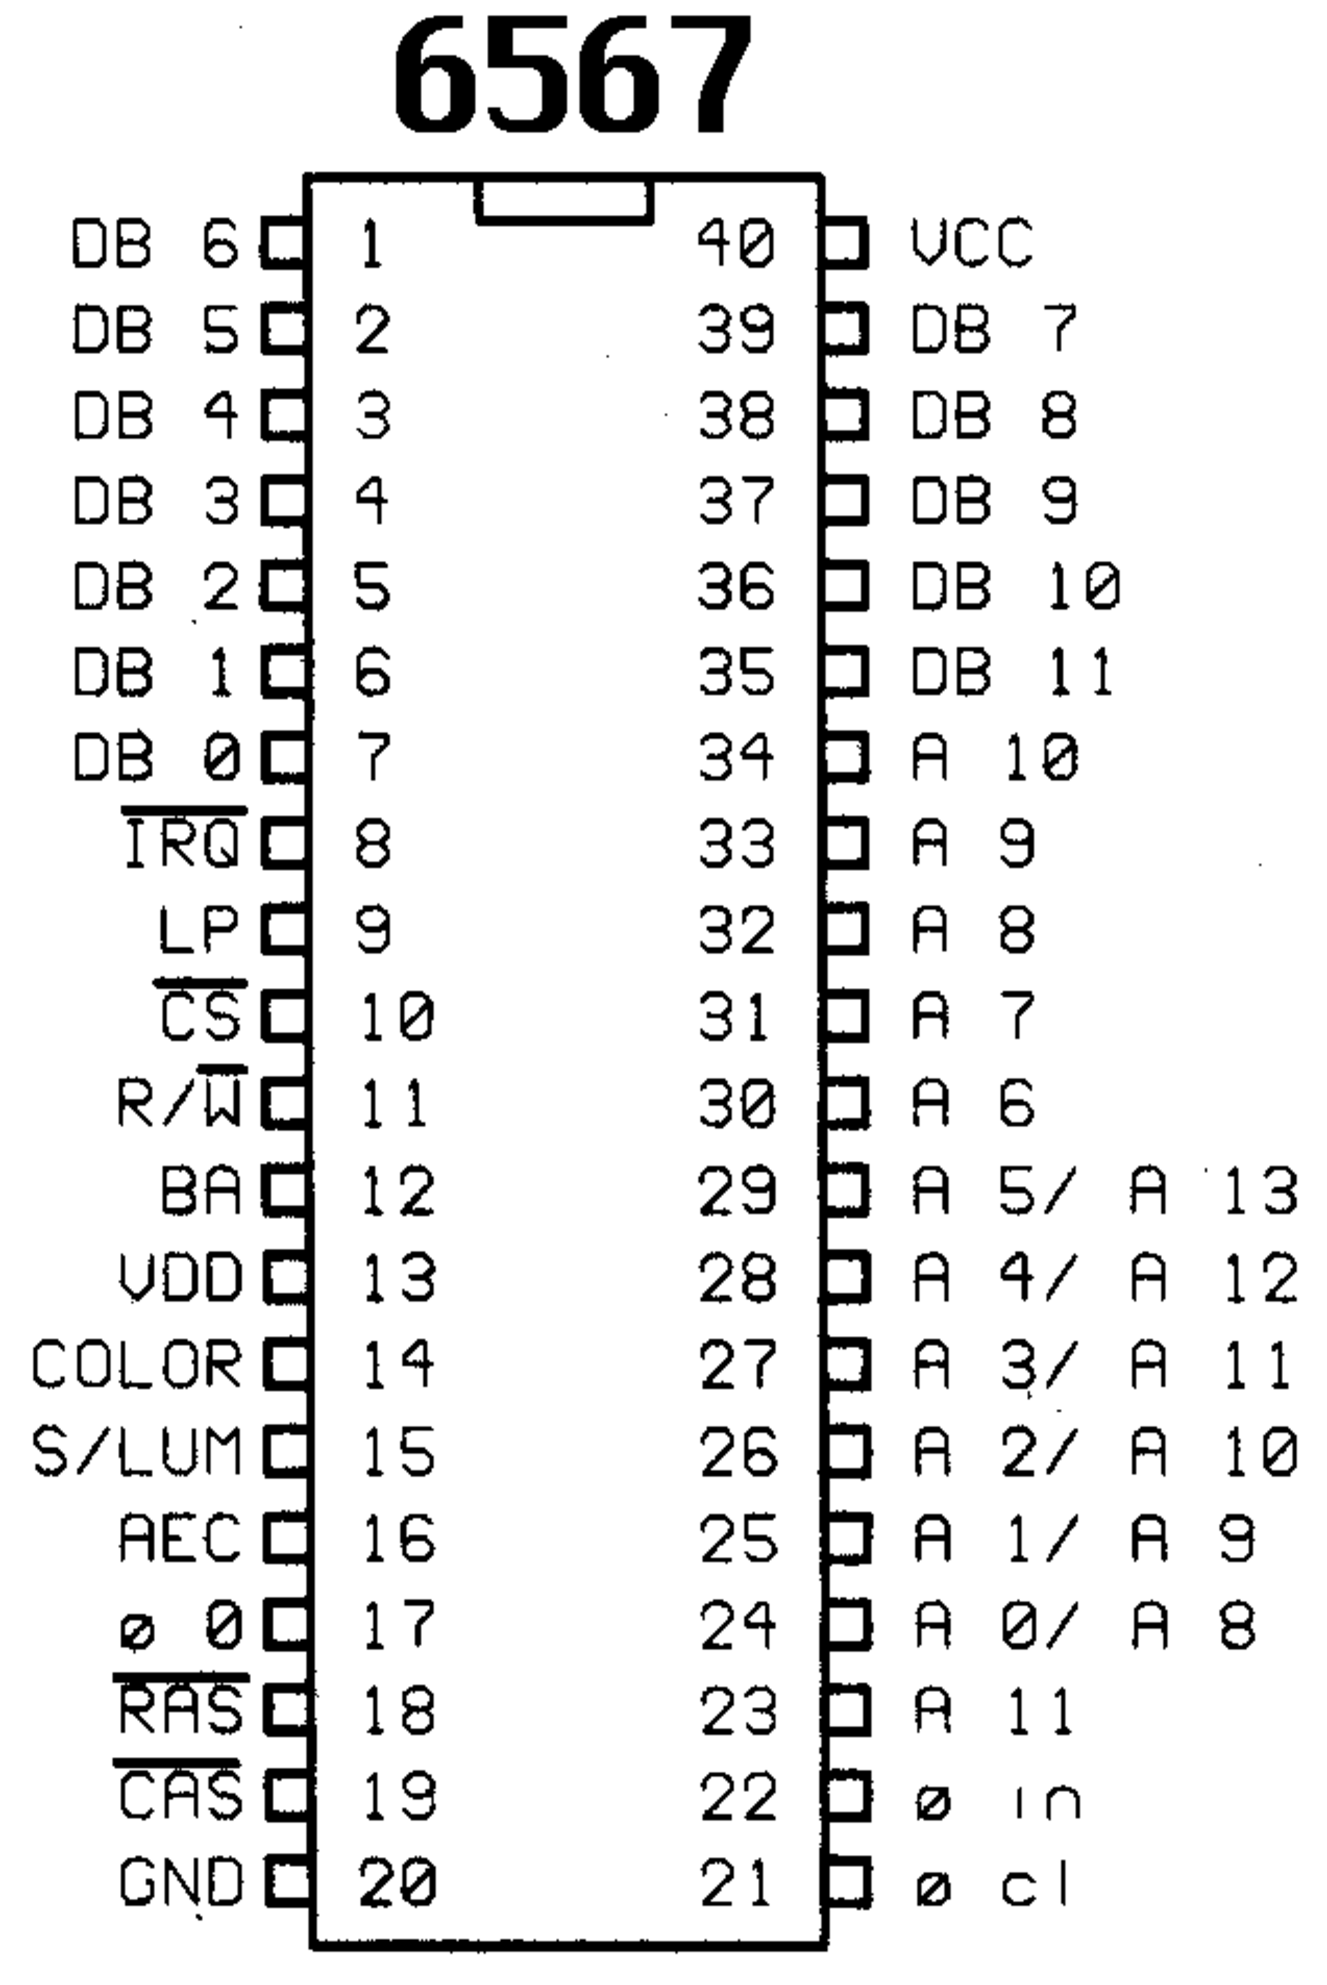
\includegraphics[width=3cm]{6567}
\caption{6567 VIC-II pin layout. Source: \cite{c64_tech_details}}
\end{center}
\end{wrapfigure}
The MOS Technology VIC-II is the device tasked with graphical output for the Commodore 64. It consists of two models, the 6567, used in NTSC chipsets, and the 6569 in the PAL ones. The chip is primarily responsible for interpreting various elements of RAM as video memory, then outputting that as composite video signals for a low-cost display, such as a CRT monitor. This section will briefly explain the VIC-II's hardware, rendering modes, and how the device is typically programmed.

\subsubsection{Device}
\paragraph{}
The VIC-II to an extent, has the most control over the Commodore 64. The clock for the 6510 CPU is fed from it, which internally has a clock divider. This is because the VIC-II must operate at a higher frequency than the 6510's 1MHz in order to properly output a PAL/NTSC signal. The VIC-II also provides the refresh clock for the Commodore 64's DRAM, allowing faster, more frequent access to render multiple sprites from memory. Also, if the video chip finds itself in need of more time to access memory, it can temporarily "stun" and halt the microprocessor and continue using the system bus. 

\paragraph{}
The VIC-II has 14 address lines to system memory, and is thus able to access up to 16KiB of memory at a time. Through bank switching with the first CIA on the Commodore 64 though, the device can access all 64KiB. There is a 12-bit bus for the VIC-II, the lower eight bits are used to access the system's main RAM, while the upper four bits are used to access Color RAM. 

\subsubsection{Rendering Modes}
\paragraph{}
Five rendering modes are available to the VIC-II, although these can generally categorized into two particular settings: text mode and bitmap mode. Text mode creates a 40x25 character display onscreen. This is what is seen when viewing the iconic Commodore BASIC interpreter. This is created with a character matrix, containing 8-bit pointers to various 8x8 pixel character glyphs in memory. These glyphs may be from CHARACTER ROM, or a custom implementation by the programmer. Bitmap mode, the alternate setting, is typically meant for rich graphical applications, such as computer games. In this mode, byte-sized character data can be drawn to the screen with various colours, as well as having sprites rendered above. The VIC-II could display up to eight independent sprites per TV scan line at a time. Combined, these techniques provided a typical environment for game and multimedia programmers at the time.

\paragraph{}
A feature the Commodore 64 specifically had for visual applications were \textit{raster interrupts}. Raster interrupts allowed the VIC-II to signal the processor to take control of memory upon reaching a certain scanline, allowing it to alter the VIC-II's registers and memory. This special feature allowed clever assembly programmers to render sprites and text simultaneously on screen, or in some cases show more than eight sprites at a time.

\subsubsection{Programming the VIC-II}
\paragraph{}
The VIC-II is manipulated through 47 various control registers, these are mapped throughout memory locations $\mathtt{\$D000 - \$D3FF}$ and repeat every 64 bytes. These control registers correspond to the various aspects of the features of the VIC-II. Examples of the register's functionality include sprite data pointers, onscreen locations, raster interrupt information, as well as color palette information. The VIC-II also contains hardware features to determine if two rendered sprites overlap each other, allowing for a sort of two-dimensional "collision detection".

\subsection{MOS 6581 SID}
\paragraph{}
The MOS Technology 6581 Sound Interface Device, or SID is the programmable sound chip used in the Commodore 64. The SID was responsible for creating a variety of synthesized audio for various multimedia applications. While the sounds of the SID are considered quite primitive by today's standards, it's worth noting that they were quite groundbreaking at their time of production. The SID was chiefly designed by Robert Yannes, who was interested in creating a synthesizer for a computer that had more sophisticated audio capabilities. This section will cover the general capabilities of the SID, and how a programmer would typically interact with it.

\subsubsection{Device Features}
\paragraph{}
\begin{wrapfigure}{l}{0.4\textwidth}
\vspace{-20pt}
\begin{center}
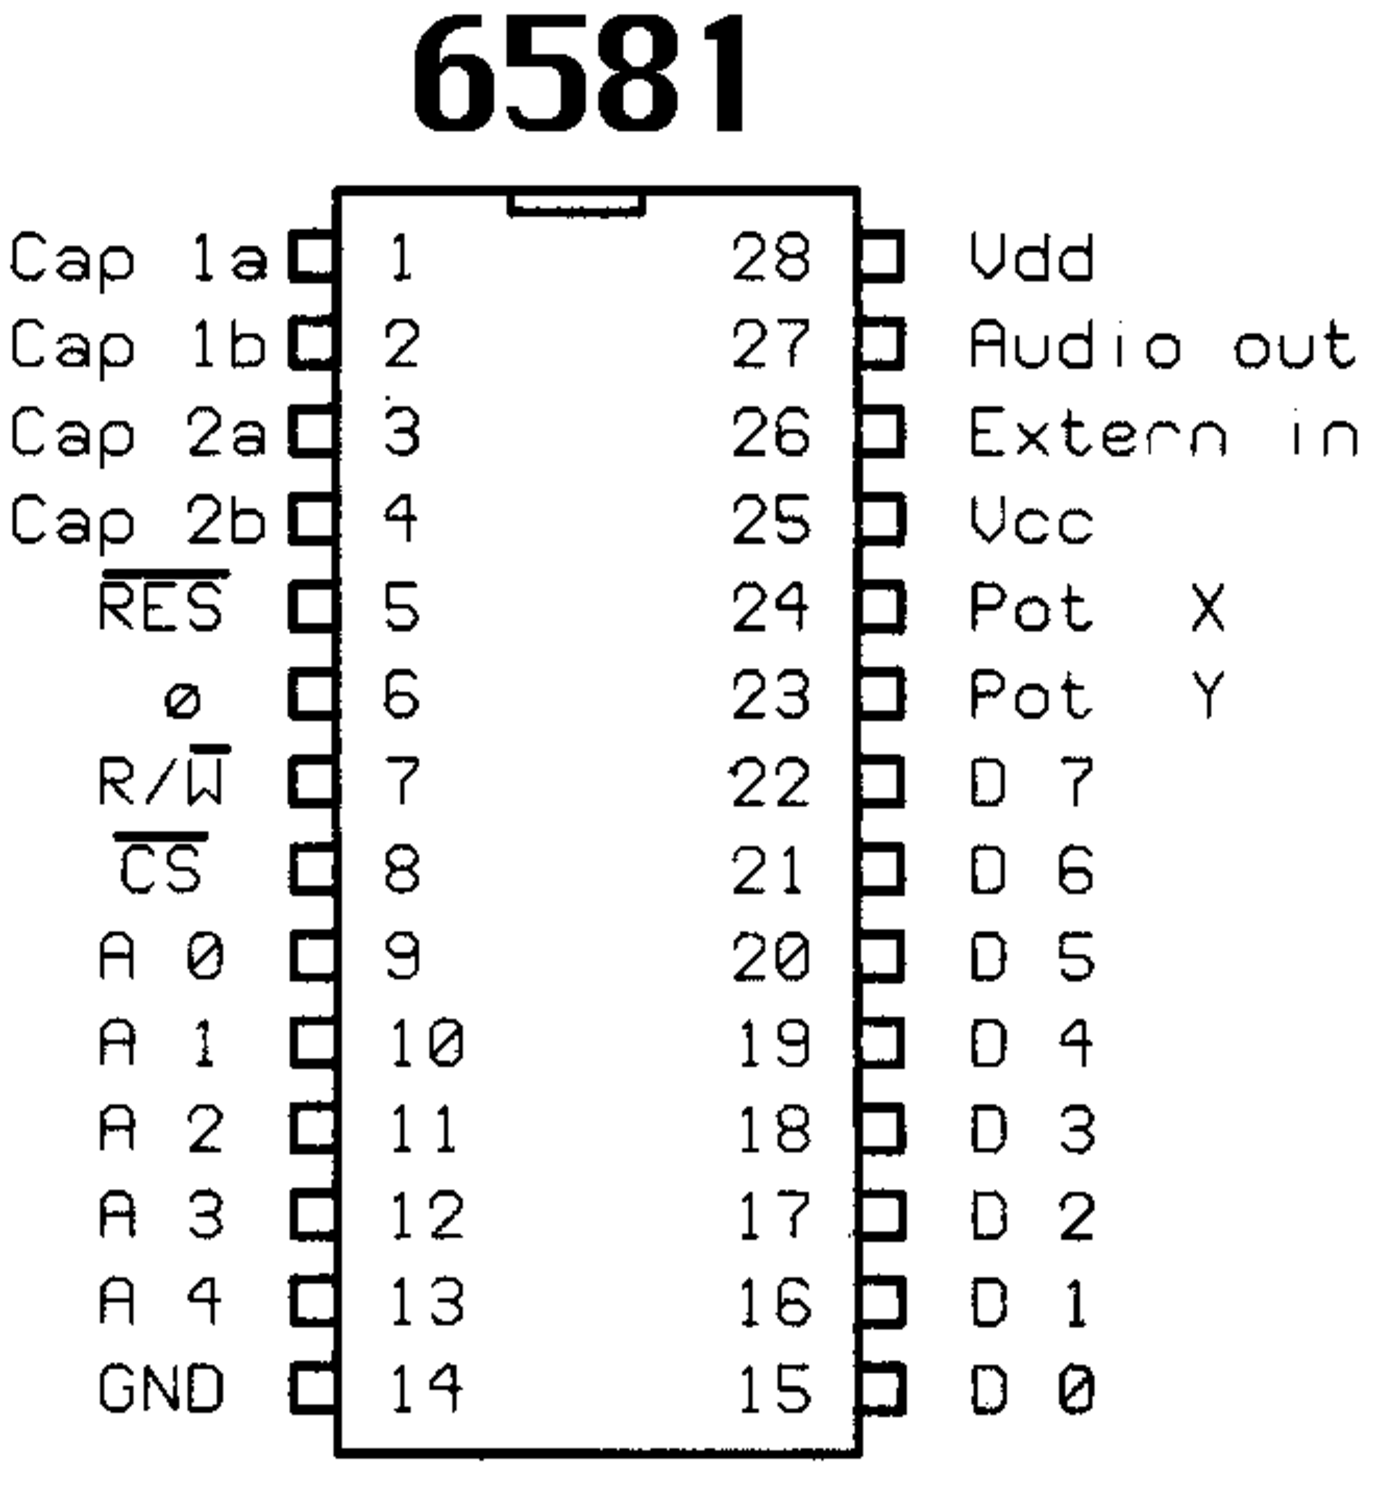
\includegraphics[width=3.5cm]{6581}
\caption{6581 SID pin layout. Source: \cite{c64_tech_details}}
\end{center}
\end{wrapfigure}
The SID's chief feature was that it allowed for three programmable distinct audio oscillators, each able to produce up to four different sound waveforms (sawtooth waves, triangle waves, pulse waves, as well as white noise). The SID was capable of commanding control of pitch, tone, and dynamics of the sounds it played. The SID also had analog-to-digital input lines, allowing for input from devices such as mice or paddles. Also due to the fact that the device is able to produce white noise, a random number generator is also provided for the 6502 to use. Random numbers and noise are generated through a 23-bit linear feedback shift register.

\paragraph{}
The 6581 was later revised and produced in later commodore models as the SID 8580, correcting some specification flaws in the original model. Interestingly enough, a number of hobbyist composers for the Commodore 64's SID find the revised model's filters produce a different sound that lacks some of the character that the original 6581 contains.

\subsubsection{Operating the SID}
Much like the VIC-II, operating the SID is done through a variety of registers available to the programmer from memory. When I/O and devices are bank switched into the address space, the SID's registers can be accessed across $\mathtt{\$D400 - \$D7FF}$. Various features of the registers include voice frequency/pulse width, volume dynamics, filter cutoff, and read-only paddle data.

\subsection{MOS 6526 CIA}
\paragraph{}
The MOS Technology 6526 CIA is the interface chip used in the Commodore 64. Two are found inside the Commodore 64 chipset. Each featured 2 8-bit I/O ports, timers, an 8-bit shift register for serial I/O, and a real-time clock for peripheral devices. It's primary purpose was to interface with the keyboard, joysticks, and external ports for serial devices. The registers for both CIAs can be found across $\mathtt{\$DC00 - \$DCFF}$ and $\mathtt{\$DD00 - \$DDFF}$.

\section{Strengths}
\paragraph{}
Arguably, one of the largest advantages of the Commodore 64 is it's simplicity, from an economic as well as a technical perspective. The 6502 microprocessor was comparatively inexpensive to produce compared to competitors such as the Intel 8080, and showed comparable performance with the correct memory configuration. Commodore's business strategy involved reducing costs where possible by producing parts in-house where possible. It's comprehensive feature set provided a viable personal computing platform at a fraction of the price.

\paragraph{}
While comprehensive, the Commodore 64 also proved a strength in it's difference from typical computers at the time thanks to its programmable nature and rich multimedia capabilities. With the powerful capabilities of the VIC-II and SID, experienced programmers could create multimedia-oriented software not found  along with the ability to hack, tune, and tweak the device effectively, the Commodore 64 proved to be a comfortable option for the consumer computer enthusiast or hobbyist. 

\section{Weaknesses}
\paragraph{}
While programmable and able to offer a great deal of power to the user, the Commodore 64 is not without its shortcomings. The device had a very fixed hardware setup, and could not particularly be expanded, upgraded, or modified easily. Users looking expand their hardware setups often had to purchase entirely new computers. Competitor devices, such as the Apple II had a variety of comprehensive expansion slots that could allow more powerful functionality. 

\section{Critical analysis \& Conclusion}
\paragraph{}
Overall, the Commodore 64 is notable example of how a significantly \textit{different} computer can be incredibly effective as a market strategy. While it may not have had the power or flexibility of certain systems, such as the Apple II, the Commodore 64 arguably gained its significant market share through marketing itself as a cheaper, easier to use, and more applicable computer for consumer usage. Its chief advantage was that it provided a comprehensive package at a fraction of the cost and complexity. Arguably, this is why, in some ways, the Commodore 64 has retained the spirit of its popularity with some hobbyists even today.

\pagebreak

\begin{thebibliography}{9}

\bibitem{c64_arch}
  \emph{C64 Hardware and Architecture}.\\
  http://www.skinfaxi.com/cli/C64/hardarch.htm
  
\bibitem{cp_wiki}
  \emph{The Commodore Programming Wiki}.\\
  http://commodore64.wikispaces.com/
  
\bibitem{blog_cp}
   \emph{A Blog from the 80's about C64 Programming}.\\
   http://c64programming.wordpress.com/

\bibitem{c64_tech_details}
   \emph{Commodore 64 - Technical Details}.\\
   MJK's Commodore 64 \& LCD Page,
   http://ist.uwaterloo.ca/\textasciitilde{}schepers/MJK/c64\_\_.html
   
\bibitem{refGuide}
   \emph{Commodore 64 Programmer's Reference Guide}.\\
   Commodore Business Machines Inc.\\
   http://www.commodore.ca/manuals/c64\_programmers\_reference/c64-programmers\_reference.htm

\bibitem{6502org}
   \emph{6502.org}.\\
   http://http://6502.org/

\bibitem{6502class}
   \emph{6502 class IC's}.\\
   cpu-collection.de\\
   http://www.cpu-collection.de/?tn=1\&l0=cl\&l1=650x

\bibitem{bestLayout}
   \emph{The MOS 6502 and the Best Layout Guy in the World}.\\
   Russ Cox\\
   research!rsc\\
   http://research.swtch.com/6502

\bibitem{reconstruction}
   \emph{Reconstruction of the MOS 6502 on the Cyclone II FPGA}.\\
   Chen, Choi, Sundaram, and Erlinger\\
   http://www.cs.columbia.edu/\textasciitilde{}sedwards/classes/2013/4840/reports/6502.pdf

\bibitem{twoClock}
   \emph{The 6502's two clock signals}.\\
   http://lateblt.livejournal.com/88105.html

\bibitem{nesProg}
   \emph{NES Programming/Introduction}.\\
   WikiBooks - NES Programming\\
   http://en.wikibooks.org/w/index.php?title=NES\_Programming/Introduction\&oldid=2364817 \\
   Current revision as of 17-02-2013

\bibitem{zeroPage}
   \emph{Zero Page}.\\
   Game Design Novice\\
   http://gamedesign.wikidot.com/6502:zero-page
   
\bibitem{easy6502}
   \emph{Easy 6502}.\\
   Nick Morgan \\
   GitHub \\
   http://skilldrick.github.io/easy6502/
   
\bibitem{opcodes}
   \emph{6502 Assembly}.\\
   WikiBooks\\
   http://en.wikibooks.org/w/index.php?title=6502\_Assembly\&oldid=2597563 \\
   Current revision as of 17-02-2013
   
\bibitem{6510sheet}
   \emph{6510 Microprocessor With I/O}.\\
   Commodore Semiconductor Group \\
   http://archive.6502.org/datasheets/mos\_6510\_mpu.pdf
   
   \bibitem{6560sheet}
   \emph{660/6561 Video Interface Chip}.\\
   Commodore Semiconductor Group \\
  http://www.mdawson.net/vic20chrome/display/mos\_6560\_6561\_vic.pdf
   
\bibitem{c64_memMap}
   \emph{Commodore 64 Memory maps}.\\
   Project 64, 1996\\
   http://unusedino.de/ec64/technical/project64/memory\_maps.html
      
\bibitem{memMap}
   \emph{Memory Map}.\\
   Commodore 64 Wiki \\
   http://www.c64-wiki.com/index.php?title=Memory\_Map\&oldid=17227
   Current revision as of 17-02-2013
      
\bibitem{}
   \emph{VIC-II Reference}.\\
   8-bit register reference
   Oxyron \\
   http://www.oxyron.de/html/registers\_vic2.html
  
   \bibitem{ars}
   \emph{Total share: 30 years of personal computer market share figures}.\\
   Jeremy Reimer, 2005 \\
   Ars Technica
   http://arstechnica.com/features/2005/12/total-share/
     
   \bibitem{caseHistory}
   \emph{Design case history: the Commodore 64}.\\
   Perry, Wallich,
   IEEE Spectrum 48-58, March 1985\\
   http://spectrum.ieee.org/ns/pdfs/commodore64\_mar1985.pdf
     
   \bibitem{wiredArticle}
   \emph{Grandiose Price for a Modest PC}.\\
   Leander Kahney
   Wired, 2003
   http://www.wired.com/culture/lifestyle/news/2003/09/60349
   
\end{thebibliography}

\end{document}